\documentclass[12pt, a4paper]{article}
\usepackage[utf8]{inputenc}
\usepackage{ragged2e}

\usepackage{graphicx, geometry, hyperref, wrapfig, amsmath, subcaption, setspace}
\usepackage[dvipsnames]{xcolor}

\definecolor{silver}{RGB}{200,200,200}
\hypersetup{colorlinks=true, linkcolor=RoyalBlue, urlcolor=RoyalBlue}

 \geometry{
 a4paper,
 total={175mm,257mm},
 left=20mm,
 top=15mm,
 }

\usepackage{xcolor} % for defining colour
\usepackage{titlesec} % for customizing sections

% \usepackage{times}        % Use Times New Roman font
% \usepackage{helvet}       % Use Helvetica font
\usepackage{palatino}

\usepackage[T1]{fontenc}

\setlength\parindent{0pt}

% %%%%%%%%%%%%%%%%%%%%%%%%%%%%%%%%%%%%%%%%%%%%%%%%%%%%%%%%%%%%%%
\titleformat{\section}
{\color{UM_DarkBlue}\normalfont\large\bfseries}
{\color{UM_DarkBlue}\thesection}{1em}{}

%%%%%%%%%%%%%%%%%%%%%%%%%%%%%%%%%%%%%%%%%%%%%%%%%%%%%%%%%%%%%%%
\definecolor{UM_Brown}{HTML}{3D190D}
\definecolor{UM_DarkBlue}{HTML}{2264B0}
\definecolor{UM_LightBlue}{HTML}{1CA9E1}
\definecolor{UM_Orange}{HTML}{fEB415}

%%%%%%%%%%%%%%%%%%%%%%%%%%%%%%%%%%%%%%%%%%%%%%%%%%%%%%%%%%%%%%%%

\newcommand{\eg}{{\it e.g.}}
\newcommand{\ie}{{\it i.e.}}

% %%%%%%%%%%%%%%%%%%%%%%%%%%%%%%%%%%%%%%%%%%%%%%%%%%%%%%%%%%%%%%
% \hypersetup{
%     draft=false,
%     final=true,
%     colorlinks=true,
%     citecolor=UM_DarkBlue,
%     anchorcolor=yellow,
%     linkcolor=UM_DarkBlue,
%     urlcolor=UM_DarkBlue,
%     filecolor=green,      
%     pdfpagemode=FullScreen,
%     bookmarksopen=false
%     }
\usepackage{amsmath,amsfonts,amssymb,bm}

%%%%%%%%%%%%%%%%%%%%%%%%%%%%%%%%%%%%%%%%%%%%%%%%%%%%%%%%%%%%%
% Sets and Notations
\newcommand{\reals}{\mathbb{R}}
\newcommand{\integers}{\mathbb{Z}}

%%%%%%%%%%%%%%%%%%%%%%%%%%%%%%%%%%%%%%%%%%%%%%%%%%%%%%%%%%%%%
% Vectors and Matrices
% \renewcommand{\vec}[1]{\bm{\mathrm{#1}}}
\newcommand{\dotp}{\,\boldsymbol{\cdot}\,}
\newcommand{\grad}[1]{\vec{\nabla}#1}
\renewcommand{\div}[1]{\vec{\nabla}\!\dotp\!\vec{#1}}
\newcommand{\curl}[1]{\vec{\nabla}\!\times\!\vec{#1}}



%%%%%%%%%%%%%%%%%%%%%%%%%%%%%%%%%%%%%%%%%%%%%%%%%%%%%%%%%%%%%
% Derivatives
\newcommand{\dv}[2]{\frac{d#1}{d#2}}
\newcommand{\ndv}[3][2]{\frac{d^{\,#1}#2}{d#3^{\,#1}}}

\newcommand{\pdv}[2]{\frac{\partial#1}{\partial#2}}
\newcommand{\npdv}[3][2]{\frac{\partial^{\,#1}#2}{\partial#3^{#1}}}
 
\title{OWO-GAship}
\author{Anik Mandal}
\date{January 2025}
\pagenumbering{arabic}
\setstretch{1.4}

%====================================================================================================
\begin{document}


\begin{minipage}[t][][c]{0.1\textwidth}
    \begin{flushleft}
        
\includegraphics[height=2cm]{tex-resources/Ashoka Logo.png}
    \end{flushleft}
\end{minipage}
\begin{minipage}[t][][c]{0.85\textwidth}
    \begin{center}
        {\LARGE Oscillations, Wave and Optics}\\ \vspace{0.5em}
        \textsc{(Spring 2025)}\\
        \vspace{1em}
        \textbf{\Large MIDTERM EXAMINATION} \\
    \end{center}
\end{minipage}
\vspace{20pt}\\
\rule[0em]{\textwidth}{0.75pt}

\flushleft{Date: 6th March, 2025}\hfill
\fbox{\textbf{\large 
Time: 90 Minutes}(15:00-16:30)}\hfill
\textbf{\large 
Mark: 21}\\

\textbf{Instructions}:
\begin{itemize}
    \item Write physics arguments and definitions clearly while arriving at the mathematical proofs.
    Unclear statements, mathematical proofs will not be considered. 
    \item You are not allowed to use any kind of study materials or books during the exam.
    (Only a scientific calculator is allowed if required)
    \item Answer any 3 problems out of 5.
\end{itemize}
\begin{center}
    \textbf{All the best!!!}
\end{center}
\rule[0em]{\textwidth}{1.75pt}
\vspace{-1cm}

%====================================================================================================
%====================================================================================================
\justifying

%#######################################
\section*{Problem-1 \hfill \textbf{[7]}}
\noindent
\textbf{(1)} If the amplitude of a damped harmonic oscillator decreases to $1/{\rm e}$ of its 
initial value after $n\gg 1$ periods show that the ratio of the period of oscillation to the period
 of the oscillation with no damping is approximately
\begin{align*}
    1 + \frac{1}{8\pi^{2}n^{2}}
\end{align*}\hfill\textbf{4}\\

\noindent
\textbf{(2)} Consider a periodic function,
\[ f(x) =
\begin{cases} 
0, & \text{for } -\pi< x < 0 \\
x, & \text{for } 0\leq x <\pi
\end{cases}
\] 

Determine the Fourier coefficients and express f(x) in terms of the Fourier series.
\hfill\textbf{3}\\


%#######################################
\begin{figure}[h]
    \centering
    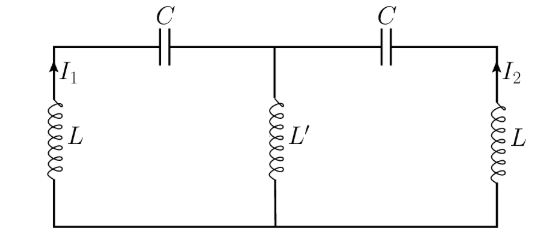
\includegraphics[scale=0.4]{figs/LC-coupled.png}
    \caption{}
    \label{fig:LC-coupled}
\end{figure}
\section*{Problem-2 \hfill \textbf{[7]}}
Find the normal frequencies and normal modes of the coupled LC circuit shown in 
Figure-\ref{fig:LC-coupled} in terms of $\omega_0=1/\sqrt{L\,C}$ and $\alpha=L'/L$.



%#######################################
\section*{Problem-3 \hfill \textbf{[7]}}
Consider a uniformly beaded string with $N$ beads that is similar to that pictured in 
Figure-\ref{fig:Nbead-ring}, except that each end of the string is attached to a massless ring that slides 
(in the $y$-direction) on a frictionless rod.
\begin{figure}[h]
    \centering
    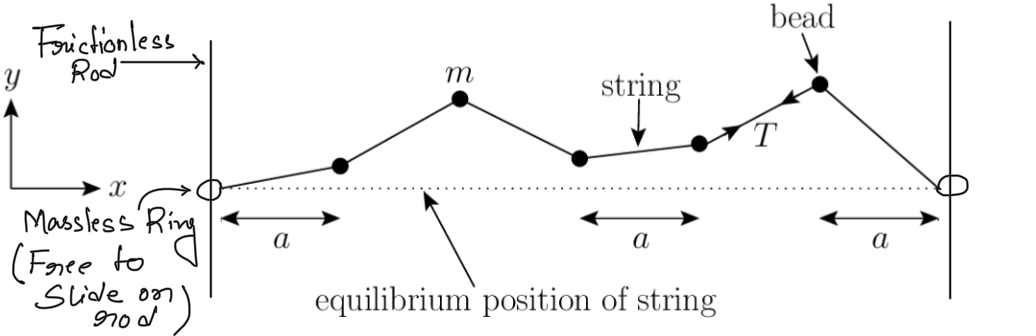
\includegraphics[scale=0.25]{figs/Nbead-ring.jpeg}
    \caption{}
    \label{fig:Nbead-ring}
\end{figure}

\textbf{i.} Demonstrate that the normal modes of the system take the form
\begin{align*}
    y_{n,i}(t) = A_n\cos\left[\frac{n(i-1/2)}{N}\pi\right]\cos(\omega_nt-\phi_n)
\end{align*}

where
\begin{align*}
    \omega_n = 2\omega_0\sin\left(\frac{n}{N}\frac{\pi}{2}\right)
\end{align*}

$\omega_0$ is defined as $\sqrt{T/ ma}$ , $A_n$ and $\phi_n$ are constants, the integer $i=1,N$ 
indexes the beads, and the mode number $n$ indexes the modes.

\textbf{ii.} How many unique normal modes does the system possess, and what are their mode numbers?

\textbf{iii.} Show that the lowest frequency mode has an infinite wavelength and zero frequency. 
Explain this peculiar result.\hfill\textbf{3+2+2}


%#######################################
\section*{Problem-4 \hfill \textbf{[7]}}
Consider a linear array of $N$ identical simple pendula of mass $m$ and length $l$ 
that are suspended from equal-height points, evenly spaced a distance $a$ apart. 
Suppose that each pendulum bob is attached to its two immediate neighbors by means 
of light springs of unstretched length $a$ and spring constant $K$. 
Figure-\ref{fig:pen-chain} shows a small part of such an array. Let $x_i=i\,a$ be
the equilibrium position of the $i$th bob, for $i=1,N$, and let $\psi_i(t)$ be its
horizontal displacement. It is assumed that $\vert\psi_i\vert/a\ll 1$ for all $i$.
\begin{figure}[h]
    \centering
    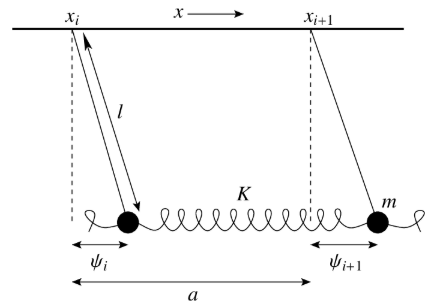
\includegraphics[scale=0.4]{figs/Pend-coupled-chain.png}
    \caption{}
    \label{fig:pen-chain}
\end{figure}\hfill\textbf{2+2+3}

\textbf{i.} Demonstrate that the equation of motion of the $i$th pendulum bob is
\begin{align*}
    \ddot{\psi}_i = - \frac{g}{l}\,\psi_i + \frac{K}{m}(\psi_{i-1}-2\psi_i+\psi_{i+1}).
\end{align*}

\textbf{ii.} Consider a general normal mode of the form
\begin{align*}
    \psi_i(t) = [A\sin (kx_i)+ B\cos(kx_i)]\cos(\omega t-\phi)
\end{align*}

Show that the associated dispersion relation is
\begin{align*}
    \omega^{2}= \frac{g}{l} + \frac{4K}{m}\sin^2(ka/2)
\end{align*}

\textbf{iii.} Suppose that the first and last pendulums in the array are attached to
immovable walls, located a horizontal distance $a$ away, by means of light springs of 
unstretched length $a$ and spring constant $K$. Find the normal modes of the system.


%#######################################
\section*{Problem-5 \hfill \textbf{[7]}}

\noindent
A lossy transmission line has a resistance per unit length ${\cal R}$,
in addition to an inductance per unit length ${\cal L}$, and a capacitance per unit length 
${\cal C}$. The resistance can be considered to be in series with the inductance.

\textbf{i.} Demonstrate that the Telegrapher's equations generalize to,
\begin{align*}
    \frac{\partial V}{\partial t} &=-\frac{1}{\cal C}\frac{\partial I}{\partial x}\\  
    \frac{\partial I}{\partial t} &=-\frac{\cal R}{\cal L} I - \frac{1}{\cal L}\frac{\partial V}{\partial x}
\end{align*}

\textbf{ii.} Derive an energy conservation equation of the form
\begin{align*}
    \frac{\partial{\cal E}}{\partial t} + \frac{\partial {\cal I}}{\partial x} =- {\cal R}I^{2}
\end{align*}

Where ${\cal E}$ is the energy per unit length along the line, and ${\cal I}$ the energy flux. 
Give expressions for ${\cal E}$ and ${\cal I}$. What does the right-hand side of the previous 
equation represent?

\textbf{iii.}Show that the current obeys the wave-diffusion equation
\begin{align*}
    \frac{\partial^{2} I}{\partial t^{2}}+ \frac{\cal R}{\cal L}\frac{\partial I}{\partial t} = \frac{1}{{\cal L}{\cal C}}\frac{\partial^{2} I}{\partial x^{2}}
\end{align*}

\textbf{iv.} Consider the low-resistance, high-frequency, limit $\omega\gg {\cal R}/{\cal L}$.
Demonstrate that a signal propagating down the line varies as
\begin{align*}
    I(x,t) &\simeq I_0\cos[k(vt-x)]{\rm e}^{-x/\delta}\\	   
    V(x,t) &\simeq Z I_0\cos[k(vt-x)-1/(k\delta)]{\rm e}^{-x/\delta}
\end{align*}

where $k=\omega/v$, $v=1/\sqrt{{\cal L}\,{\cal C}}$, $\delta = 2\,Z/{\cal R}$, 
and $Z=\sqrt{{\cal L}/{\cal C}}$. Show that $k\,\delta \gg 1$; that is, 
the decay length of the signal is much longer than its wavelength. 
Estimate the maximum useful length of a low-resistance, high-frequency, lossy transmission line.
\hfill\textbf{2+1+1+3}\\



\end{document}